\subsection{Vehicle measurements}
\label{sec:vehicle}

During this last measurement, I wanted to test our converter under
the conditions of in vivo vehicle measurements. The great advantage in
this setting is, that the European guidelines for nitrogen oxide
emission (the so called Euro 6 norms) are only concerned with \ch{NO_x}
(c.\,f.~\cite{eu}), i.\,e.\ in this case it is not necessary to separate
\ch{NO} from \ch{NO2}. Still I wanted to compare our \ch{NO_x}
results to the results of pure \ch{NO2} measurements to gauge the
influence of the additional \ch{NO} on the air pollution. Therefore
two cavities were used in parallel. One with the converter, the
other one without. With this very comfortable setup, I could even
compute the \ch{NO} concentration without having to switch the ozone,
which mitigated all the undesired effects described in the previous
two sections.

\subsubsection{Setup}
\label{sec:vehicle-setup}

For the measurement, a car was loaded with both cavities and the
pickup tube ended directly above the front license plate. The
\ch{NO_x} cavity was setup according to Section~\ref{sec:inclusion}
with an exposure time of \SI{10}{\milli\second} and 1000 scans per
spectrum leading to a time resolution of \SI{1}{\second}. As \ch{NO2}
cavity I used the AQM$_{\text{Tec}}$ Compact Cavity, which is the
standard cavity at the Institute for Environmental Physics for
\ch{NO2} measurements in urban areas and especially vehicle
measurements. This cavity operated at a \SI{2}{\second} time
resolution and had the further advantage of possessing a \ch{CO2}
sensor. This allowed us to compute ratios between nitrogen (di-)oxide
and carbon dioxide, which is a good measure for the emission per
(gazoline) consumption.

The measurements took place on Friday, February 05, 2016 in Heidelberg
between 11:00 and 16:30. From 12:15 to 13:45, I operated both
cavities in \ch{NO2} mode to test for systematic deviations. From
15:00 to 16:00, I positioned our measurement vehicle next to the
Heidelberg air quality measurement station to be able to compare our
\ch{NO} and \ch{NO2} values to the ones of the station as a test of
reliability. In between 30 vehicles were observed throughout
Heidelberg for {\nfrac{} 1/2}~\si{\minute} to \SI{10}{\minute} each
and tried to stay within their exhaust plume. Since the two cavities'
clocks could not be fully synchronized, the time series had to be
matched in the evaluation process. This was done manually using succinct
peaks in the plots.

\begin{figure}[htbp]
  \centering
  % GNUPLOT: LaTeX picture with Postscript
\begingroup
  \makeatletter
  \providecommand\color[2][]{%
    \GenericError{(gnuplot) \space\space\space\@spaces}{%
      Package color not loaded in conjunction with
      terminal option `colourtext'%
    }{See the gnuplot documentation for explanation.%
    }{Either use 'blacktext' in gnuplot or load the package
      color.sty in LaTeX.}%
    \renewcommand\color[2][]{}%
  }%
  \providecommand\includegraphics[2][]{%
    \GenericError{(gnuplot) \space\space\space\@spaces}{%
      Package graphicx or graphics not loaded%
    }{See the gnuplot documentation for explanation.%
    }{The gnuplot epslatex terminal needs graphicx.sty or graphics.sty.}%
    \renewcommand\includegraphics[2][]{}%
  }%
  \providecommand\rotatebox[2]{#2}%
  \@ifundefined{ifGPcolor}{%
    \newif\ifGPcolor
    \GPcolorfalse
  }{}%
  \@ifundefined{ifGPblacktext}{%
    \newif\ifGPblacktext
    \GPblacktexttrue
  }{}%
  % define a \g@addto@macro without @ in the name:
  \let\gplgaddtomacro\g@addto@macro
  % define empty templates for all commands taking text:
  \gdef\gplbacktext{}%
  \gdef\gplfronttext{}%
  \makeatother
  \ifGPblacktext
    % no textcolor at all
    \def\colorrgb#1{}%
    \def\colorgray#1{}%
  \else
    % gray or color?
    \ifGPcolor
      \def\colorrgb#1{\color[rgb]{#1}}%
      \def\colorgray#1{\color[gray]{#1}}%
      \expandafter\def\csname LTw\endcsname{\color{white}}%
      \expandafter\def\csname LTb\endcsname{\color{black}}%
      \expandafter\def\csname LTa\endcsname{\color{black}}%
      \expandafter\def\csname LT0\endcsname{\color[rgb]{1,0,0}}%
      \expandafter\def\csname LT1\endcsname{\color[rgb]{0,1,0}}%
      \expandafter\def\csname LT2\endcsname{\color[rgb]{0,0,1}}%
      \expandafter\def\csname LT3\endcsname{\color[rgb]{1,0,1}}%
      \expandafter\def\csname LT4\endcsname{\color[rgb]{0,1,1}}%
      \expandafter\def\csname LT5\endcsname{\color[rgb]{1,1,0}}%
      \expandafter\def\csname LT6\endcsname{\color[rgb]{0,0,0}}%
      \expandafter\def\csname LT7\endcsname{\color[rgb]{1,0.3,0}}%
      \expandafter\def\csname LT8\endcsname{\color[rgb]{0.5,0.5,0.5}}%
    \else
      % gray
      \def\colorrgb#1{\color{black}}%
      \def\colorgray#1{\color[gray]{#1}}%
      \expandafter\def\csname LTw\endcsname{\color{white}}%
      \expandafter\def\csname LTb\endcsname{\color{black}}%
      \expandafter\def\csname LTa\endcsname{\color{black}}%
      \expandafter\def\csname LT0\endcsname{\color{black}}%
      \expandafter\def\csname LT1\endcsname{\color{black}}%
      \expandafter\def\csname LT2\endcsname{\color{black}}%
      \expandafter\def\csname LT3\endcsname{\color{black}}%
      \expandafter\def\csname LT4\endcsname{\color{black}}%
      \expandafter\def\csname LT5\endcsname{\color{black}}%
      \expandafter\def\csname LT6\endcsname{\color{black}}%
      \expandafter\def\csname LT7\endcsname{\color{black}}%
      \expandafter\def\csname LT8\endcsname{\color{black}}%
    \fi
  \fi
    \setlength{\unitlength}{0.0500bp}%
    \ifx\gptboxheight\undefined%
      \newlength{\gptboxheight}%
      \newlength{\gptboxwidth}%
      \newsavebox{\gptboxtext}%
    \fi%
    \setlength{\fboxrule}{0.5pt}%
    \setlength{\fboxsep}{1pt}%
\begin{picture}(7776.00,4320.00)%
    \gplgaddtomacro\gplbacktext{%
      \csname LTb\endcsname%
      \put(682,440){\makebox(0,0)[r]{\strut{}$10$}}%
      \put(682,892){\makebox(0,0)[r]{\strut{}$20$}}%
      \put(682,1344){\makebox(0,0)[r]{\strut{}$30$}}%
      \put(682,1796){\makebox(0,0)[r]{\strut{}$40$}}%
      \put(682,2248){\makebox(0,0)[r]{\strut{}$50$}}%
      \put(682,2699){\makebox(0,0)[r]{\strut{}$60$}}%
      \put(682,3151){\makebox(0,0)[r]{\strut{}$70$}}%
      \put(682,3603){\makebox(0,0)[r]{\strut{}$80$}}%
      \put(682,4055){\makebox(0,0)[r]{\strut{}$90$}}%
      \put(814,220){\makebox(0,0){\strut{}12:10}}%
      \put(1471,220){\makebox(0,0){\strut{}12:20}}%
      \put(2127,220){\makebox(0,0){\strut{}12:30}}%
      \put(2784,220){\makebox(0,0){\strut{}12:40}}%
      \put(3440,220){\makebox(0,0){\strut{}12:50}}%
      \put(4097,220){\makebox(0,0){\strut{}13:00}}%
      \put(4753,220){\makebox(0,0){\strut{}13:10}}%
      \put(5410,220){\makebox(0,0){\strut{}13:20}}%
      \put(6066,220){\makebox(0,0){\strut{}13:30}}%
      \put(6723,220){\makebox(0,0){\strut{}13:40}}%
      \put(7379,220){\makebox(0,0){\strut{}13:50}}%
    }%
    \gplgaddtomacro\gplfronttext{%
      \csname LTb\endcsname%
      \put(176,2247){\rotatebox{-270}{\makebox(0,0){\strut{}Concentration [ppb]}}}%
      \csname LTb\endcsname%
      \put(6392,3882){\makebox(0,0)[r]{\strut{}\text{\ch{NO2} of ICAD \ch{NO2} CE-DOAS}}}%
      \csname LTb\endcsname%
      \put(6392,3662){\makebox(0,0)[r]{\strut{}\text{\ch{NO2} of ICAD \ch{NO_x} CE-DOAS}}}%
    }%
    \gplbacktext
    \put(0,0){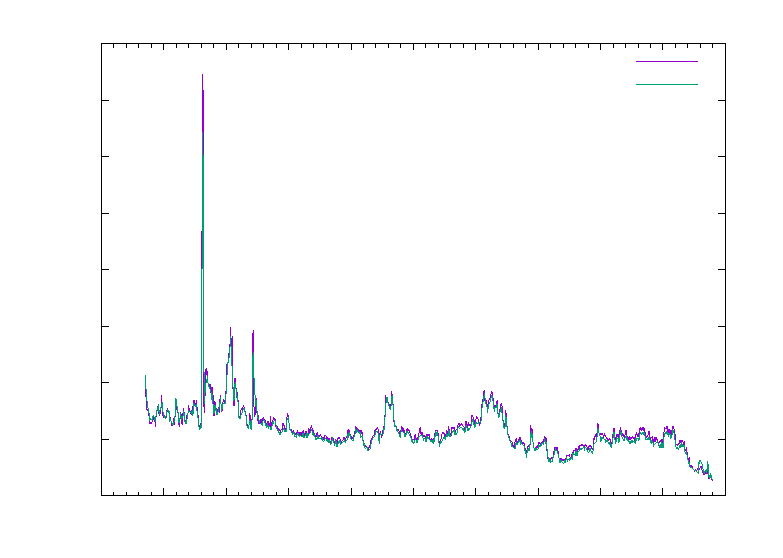
\includegraphics{../images/hd_comparison}}%
    \gplfronttext
  \end{picture}%
\endgroup

  \caption{Comparison of the two used CE-DOAS systems. Both were
    operated in pure \ch{NO2} measurement mode. The difference is
    \SI{0.43 \pm 0.01}{ppb}.}
  \label{fig:hd-comparison}
\end{figure}

\subsubsection{Results}
\label{sec:vehicle-results}

In Figure~\ref{fig:hd-comparison} one can see the comparison of the
measured \ch{NO2} concentrations of the two used cavities. It is
clearly visible that ther is no qualitative difference between the
two. However, our \ch{NO_x} cavity measured slightly lower
concentrations than the \ch{NO2} cavity with a mean difference of
$\Delta = \SI{0.43\pm0.01}{ppb}$. Absolutely speaking this is not a
large difference, but the question remains why it exists at all. The
most probable explanation is that the used zero air spectrum of the
\ch{NO_x} cavity was not completely trace gas free. One reason that
points towards this direction is, that in the \ch{NO_x} measurement
mode, there is a constant flow through the zero air input, as this is
the input for the ozone generator, too. Thus the zero air filter is much
more strained than it would be in a cavity without \ch{NO_x}
mode. Since the cavity had been thoroughly tested for multiple
Ieks, a saturation or starting effects of a saturation of
the Silica gel or the activated carbon seem plausible.

For the comparison to the air quality measurement station, this effect
might be of interest as thedeviation is large enough in this
case. During the vehicle measurements it should well be negligible as
the measured concentrations lay in the region of several hundered
\si{ppb} (see below). Additionally, the value is small compared to
other uncertainties affecting the concentrations there (e.\,g.\ the
influence of the varying distance to the measured vehicle or of the
neighbouring traffic).

\begin{figure}[htbp]
  \centering
  % GNUPLOT: LaTeX picture with Postscript
\begingroup
  \makeatletter
  \providecommand\color[2][]{%
    \GenericError{(gnuplot) \space\space\space\@spaces}{%
      Package color not loaded in conjunction with
      terminal option `colourtext'%
    }{See the gnuplot documentation for explanation.%
    }{Either use 'blacktext' in gnuplot or load the package
      color.sty in LaTeX.}%
    \renewcommand\color[2][]{}%
  }%
  \providecommand\includegraphics[2][]{%
    \GenericError{(gnuplot) \space\space\space\@spaces}{%
      Package graphicx or graphics not loaded%
    }{See the gnuplot documentation for explanation.%
    }{The gnuplot epslatex terminal needs graphicx.sty or graphics.sty.}%
    \renewcommand\includegraphics[2][]{}%
  }%
  \providecommand\rotatebox[2]{#2}%
  \@ifundefined{ifGPcolor}{%
    \newif\ifGPcolor
    \GPcolorfalse
  }{}%
  \@ifundefined{ifGPblacktext}{%
    \newif\ifGPblacktext
    \GPblacktexttrue
  }{}%
  % define a \g@addto@macro without @ in the name:
  \let\gplgaddtomacro\g@addto@macro
  % define empty templates for all commands taking text:
  \gdef\gplbacktext{}%
  \gdef\gplfronttext{}%
  \makeatother
  \ifGPblacktext
    % no textcolor at all
    \def\colorrgb#1{}%
    \def\colorgray#1{}%
  \else
    % gray or color?
    \ifGPcolor
      \def\colorrgb#1{\color[rgb]{#1}}%
      \def\colorgray#1{\color[gray]{#1}}%
      \expandafter\def\csname LTw\endcsname{\color{white}}%
      \expandafter\def\csname LTb\endcsname{\color{black}}%
      \expandafter\def\csname LTa\endcsname{\color{black}}%
      \expandafter\def\csname LT0\endcsname{\color[rgb]{1,0,0}}%
      \expandafter\def\csname LT1\endcsname{\color[rgb]{0,1,0}}%
      \expandafter\def\csname LT2\endcsname{\color[rgb]{0,0,1}}%
      \expandafter\def\csname LT3\endcsname{\color[rgb]{1,0,1}}%
      \expandafter\def\csname LT4\endcsname{\color[rgb]{0,1,1}}%
      \expandafter\def\csname LT5\endcsname{\color[rgb]{1,1,0}}%
      \expandafter\def\csname LT6\endcsname{\color[rgb]{0,0,0}}%
      \expandafter\def\csname LT7\endcsname{\color[rgb]{1,0.3,0}}%
      \expandafter\def\csname LT8\endcsname{\color[rgb]{0.5,0.5,0.5}}%
    \else
      % gray
      \def\colorrgb#1{\color{black}}%
      \def\colorgray#1{\color[gray]{#1}}%
      \expandafter\def\csname LTw\endcsname{\color{white}}%
      \expandafter\def\csname LTb\endcsname{\color{black}}%
      \expandafter\def\csname LTa\endcsname{\color{black}}%
      \expandafter\def\csname LT0\endcsname{\color{black}}%
      \expandafter\def\csname LT1\endcsname{\color{black}}%
      \expandafter\def\csname LT2\endcsname{\color{black}}%
      \expandafter\def\csname LT3\endcsname{\color{black}}%
      \expandafter\def\csname LT4\endcsname{\color{black}}%
      \expandafter\def\csname LT5\endcsname{\color{black}}%
      \expandafter\def\csname LT6\endcsname{\color{black}}%
      \expandafter\def\csname LT7\endcsname{\color{black}}%
      \expandafter\def\csname LT8\endcsname{\color{black}}%
    \fi
  \fi
    \setlength{\unitlength}{0.0500bp}%
    \ifx\gptboxheight\undefined%
      \newlength{\gptboxheight}%
      \newlength{\gptboxwidth}%
      \newsavebox{\gptboxtext}%
    \fi%
    \setlength{\fboxrule}{0.5pt}%
    \setlength{\fboxsep}{1pt}%
\begin{picture}(7200.00,5040.00)%
    \gplgaddtomacro\gplbacktext{%
      \csname LTb\endcsname%
      \put(814,440){\makebox(0,0)[r]{\strut{}$-10$}}%
      \put(814,922){\makebox(0,0)[r]{\strut{}$0$}}%
      \put(814,1403){\makebox(0,0)[r]{\strut{}$10$}}%
      \put(814,1885){\makebox(0,0)[r]{\strut{}$20$}}%
      \put(814,2367){\makebox(0,0)[r]{\strut{}$30$}}%
      \put(814,2848){\makebox(0,0)[r]{\strut{}$40$}}%
      \put(814,3330){\makebox(0,0)[r]{\strut{}$50$}}%
      \put(814,3812){\makebox(0,0)[r]{\strut{}$60$}}%
      \put(814,4293){\makebox(0,0)[r]{\strut{}$70$}}%
      \put(814,4775){\makebox(0,0)[r]{\strut{}$80$}}%
      \put(946,220){\makebox(0,0){\strut{}14:50}}%
      \put(1597,220){\makebox(0,0){\strut{}15:00}}%
      \put(2248,220){\makebox(0,0){\strut{}15:10}}%
      \put(2898,220){\makebox(0,0){\strut{}15:20}}%
      \put(3549,220){\makebox(0,0){\strut{}15:30}}%
      \put(4200,220){\makebox(0,0){\strut{}15:40}}%
      \put(4851,220){\makebox(0,0){\strut{}15:50}}%
      \put(5501,220){\makebox(0,0){\strut{}16:00}}%
      \put(6152,220){\makebox(0,0){\strut{}16:10}}%
      \put(6803,220){\makebox(0,0){\strut{}16:20}}%
    }%
    \gplgaddtomacro\gplfronttext{%
      \csname LTb\endcsname%
      \put(176,2607){\rotatebox{-270}{\makebox(0,0){\strut{}Concentration [ppb]}}}%
      \csname LTb\endcsname%
      \put(5816,4602){\makebox(0,0)[r]{\strut{}\ch{NO2}}}%
      \csname LTb\endcsname%
      \put(5816,4382){\makebox(0,0)[r]{\strut{}\ch{NO_x}}}%
      \csname LTb\endcsname%
      \put(5816,4162){\makebox(0,0)[r]{\strut{}\ch{NO_{\text{\hphantom{x}}}}}}%
    }%
    \gplbacktext
    \put(0,0){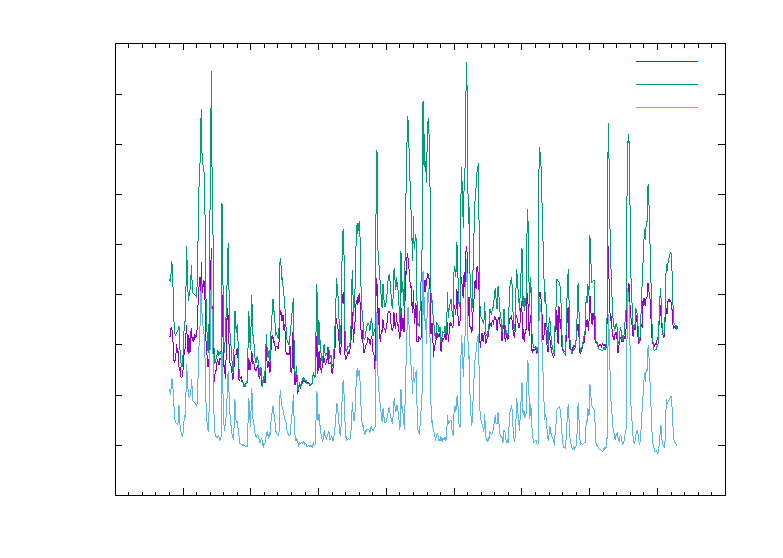
\includegraphics{../images/umba_ts}}%
    \gplfronttext
  \end{picture}%
\endgroup

  \caption{Timeseries of the \ch{NO_x}, \ch{NO2} and the computed
    \ch{NO} concentration next to the Umweltlandesamt air quality
    measurement station in Heidelberg.}
  \label{fig:umba}
\end{figure}

Figure~\ref{fig:umba} contains the time series of the measured
\ch{NO_x} and \ch{NO_2} and the computed \ch{NO} during our stay next
to the Heidelberg air quality measurement station. For moderate
\ch{NO2} concentrations between \num{10} and \SI{20}{ppb} the
\ch{NO_x} curve almost coincides with the \ch{NO2} curve. Only during
peaks there is a stronger separation and the \ch{NO_x} concentration
rises occasionally twice as high as the \ch{NO2} concentration. The
time series makes clear that neglecting \ch{NO} values while
estimating \ch{NO_x} pollution in urban areas can lead to serious
underestimation.

In a next step I computed the average concentrations for all three
time series and compared them to the station data taken
from~\cite{umba}. The results can be found in Table~\ref{tab:umba}. It
shows that there is a systematic deviation from the station, but our
values lie in the same region. The standard CE-DOAS method has been
thoroughly tested during the last decades and is known to produce
solid results in good agreement with the measurement stations. Thus
the deviation of the \ch{NO2} average points towards outer influences
as explanations for the deviation. Indeed our pickup tube was about
\SI{3}{\meter} away from the station inlet and approximately
\SI{1}{\meter} lower (which means also closer to the driving
surface). These differences in the exact location can easily account
for our measured derivations.

Nevertheless, the main result remains that under field conditions in
ambient air our measured \ch{NO_x} or respectively computed \ch{NO}
values are comparable to the ones of the station, thus indicating once
more that our converter works and that if there is a second cavity at
hand the setup seems to work very well for indirect \ch{NO}
measurements. Still some more (and longer) measurements would be
advisable to aquire more data points for enough statistics to make a
comparison between the converter method and other established \ch{NO}
measurement methods resilient.

\begin{table}[htbp]
  \centering
  \sisetup{
    table-format=2.1(2)
  }
  \begin{tabular}{l S S}
    \toprule
    {Compound} & \multicolumn{2}{c}{Concentration in \si{ppb}}\\
    & {Station} & {DOAS}\\
    \midrule
    \ch{NO} & 7.4 & 6.5 \pm 0.2\\
    \ch{NO2} & 19.2 & 21.9 \pm 0.1\\
    \ch{NOx} & 26.6 & 28.2 \pm 0.4\\ 
    \bottomrule
  \end{tabular}
  \caption{Comparison of the \SI{1}{\hour} \ch{NO}, \ch{NO2} and
    \ch{NO_x} averages from 15:00 to 16:00 on February 05, 2016
    between the air quality measurement station and the improved CE-DOAS
    instrument. The station data was taken from~\cite{umba}; no
    uncertainties were provided.}
  \label{tab:umba}
\end{table}

In between the above described experiments, \num{30} vehicles were
measured within Heidelberg. The main result is that there is a large
discrepancy between the \ch{NO2} and \ch{NO_x} values. During peaks
the \ch{NO_x} values exceed the \ch{NO2} values by far.

As an in depth analysis of all vehicles would most likely go beyond
the scope of this thesis and furthermore miss the point of
characterising and analyzing our converter, I will restrict my
attention to two vehicles. I chose these by reason of pursuit time and
distinguishability from background and ended up with one Diesel car
and a public-transit bus. These will be discussed in detail below.
The first example is a Mercedes B180 CDI.\@ The time series is
depicted in Figure~\ref{fig:mercedes-ts} and a picture of the vehicle
together with the surrounding traffic is shown in Figure~\ref{fig:bus}
left hand side. There are 5 to 6 acceleration periods visible and most
prominent in the \ch{NO_x} time series. The \ch{NO_2} values vary the
least and are between a factor 4 and a factor 9 smaller than the
\ch{NO_x} values during peaks. In the valleys between peaks, the
\ch{NO_x} approaches the \ch{NO2}, but is still significantly
higher. The \ch{CO2} time series has the same overall appearance as
the \ch{NO_x} curve. For a quantitave analysis, the nitrogen
(di-)oxide emission per carbon dioxide emission is computed. The
results can be found in Table~\ref{tab:mercedes-bus}. It shows that
there is one order of magnitude difference between the two ratios,
which again underlines the blatant underestimation of the vehicle
emissions if only \ch{NO2} values are taken into account.

\begin{figure}[htbp]
  \centering
  % GNUPLOT: LaTeX picture with Postscript
\begingroup
  \makeatletter
  \providecommand\color[2][]{%
    \GenericError{(gnuplot) \space\space\space\@spaces}{%
      Package color not loaded in conjunction with
      terminal option `colourtext'%
    }{See the gnuplot documentation for explanation.%
    }{Either use 'blacktext' in gnuplot or load the package
      color.sty in LaTeX.}%
    \renewcommand\color[2][]{}%
  }%
  \providecommand\includegraphics[2][]{%
    \GenericError{(gnuplot) \space\space\space\@spaces}{%
      Package graphicx or graphics not loaded%
    }{See the gnuplot documentation for explanation.%
    }{The gnuplot epslatex terminal needs graphicx.sty or graphics.sty.}%
    \renewcommand\includegraphics[2][]{}%
  }%
  \providecommand\rotatebox[2]{#2}%
  \@ifundefined{ifGPcolor}{%
    \newif\ifGPcolor
    \GPcolorfalse
  }{}%
  \@ifundefined{ifGPblacktext}{%
    \newif\ifGPblacktext
    \GPblacktexttrue
  }{}%
  % define a \g@addto@macro without @ in the name:
  \let\gplgaddtomacro\g@addto@macro
  % define empty templates for all commands taking text:
  \gdef\gplbacktext{}%
  \gdef\gplfronttext{}%
  \makeatother
  \ifGPblacktext
    % no textcolor at all
    \def\colorrgb#1{}%
    \def\colorgray#1{}%
  \else
    % gray or color?
    \ifGPcolor
      \def\colorrgb#1{\color[rgb]{#1}}%
      \def\colorgray#1{\color[gray]{#1}}%
      \expandafter\def\csname LTw\endcsname{\color{white}}%
      \expandafter\def\csname LTb\endcsname{\color{black}}%
      \expandafter\def\csname LTa\endcsname{\color{black}}%
      \expandafter\def\csname LT0\endcsname{\color[rgb]{1,0,0}}%
      \expandafter\def\csname LT1\endcsname{\color[rgb]{0,1,0}}%
      \expandafter\def\csname LT2\endcsname{\color[rgb]{0,0,1}}%
      \expandafter\def\csname LT3\endcsname{\color[rgb]{1,0,1}}%
      \expandafter\def\csname LT4\endcsname{\color[rgb]{0,1,1}}%
      \expandafter\def\csname LT5\endcsname{\color[rgb]{1,1,0}}%
      \expandafter\def\csname LT6\endcsname{\color[rgb]{0,0,0}}%
      \expandafter\def\csname LT7\endcsname{\color[rgb]{1,0.3,0}}%
      \expandafter\def\csname LT8\endcsname{\color[rgb]{0.5,0.5,0.5}}%
    \else
      % gray
      \def\colorrgb#1{\color{black}}%
      \def\colorgray#1{\color[gray]{#1}}%
      \expandafter\def\csname LTw\endcsname{\color{white}}%
      \expandafter\def\csname LTb\endcsname{\color{black}}%
      \expandafter\def\csname LTa\endcsname{\color{black}}%
      \expandafter\def\csname LT0\endcsname{\color{black}}%
      \expandafter\def\csname LT1\endcsname{\color{black}}%
      \expandafter\def\csname LT2\endcsname{\color{black}}%
      \expandafter\def\csname LT3\endcsname{\color{black}}%
      \expandafter\def\csname LT4\endcsname{\color{black}}%
      \expandafter\def\csname LT5\endcsname{\color{black}}%
      \expandafter\def\csname LT6\endcsname{\color{black}}%
      \expandafter\def\csname LT7\endcsname{\color{black}}%
      \expandafter\def\csname LT8\endcsname{\color{black}}%
    \fi
  \fi
    \setlength{\unitlength}{0.0500bp}%
    \ifx\gptboxheight\undefined%
      \newlength{\gptboxheight}%
      \newlength{\gptboxwidth}%
      \newsavebox{\gptboxtext}%
    \fi%
    \setlength{\fboxrule}{0.5pt}%
    \setlength{\fboxsep}{1pt}%
\begin{picture}(7200.00,5040.00)%
    \gplgaddtomacro\gplbacktext{%
      \csname LTb\endcsname%
      \put(946,966){\makebox(0,0)[r]{\strut{}$0$}}%
      \put(946,1347){\makebox(0,0)[r]{\strut{}$100$}}%
      \put(946,1728){\makebox(0,0)[r]{\strut{}$200$}}%
      \put(946,2109){\makebox(0,0)[r]{\strut{}$300$}}%
      \put(946,2490){\makebox(0,0)[r]{\strut{}$400$}}%
      \put(946,2871){\makebox(0,0)[r]{\strut{}$500$}}%
      \put(946,3251){\makebox(0,0)[r]{\strut{}$600$}}%
      \put(946,3632){\makebox(0,0)[r]{\strut{}$700$}}%
      \put(946,4013){\makebox(0,0)[r]{\strut{}$800$}}%
      \put(946,4394){\makebox(0,0)[r]{\strut{}$900$}}%
      \put(946,4775){\makebox(0,0)[r]{\strut{}$1000$}}%
      \put(1078,834){\rotatebox{-45}{\makebox(0,0)[l]{\strut{}11:15:00}}}%
      \put(1471,834){\rotatebox{-45}{\makebox(0,0)[l]{\strut{}11:15:30}}}%
      \put(1864,834){\rotatebox{-45}{\makebox(0,0)[l]{\strut{}11:16:00}}}%
      \put(2256,834){\rotatebox{-45}{\makebox(0,0)[l]{\strut{}11:16:30}}}%
      \put(2649,834){\rotatebox{-45}{\makebox(0,0)[l]{\strut{}11:17:00}}}%
      \put(3042,834){\rotatebox{-45}{\makebox(0,0)[l]{\strut{}11:17:30}}}%
      \put(3435,834){\rotatebox{-45}{\makebox(0,0)[l]{\strut{}11:18:00}}}%
      \put(3827,834){\rotatebox{-45}{\makebox(0,0)[l]{\strut{}11:18:30}}}%
      \put(4220,834){\rotatebox{-45}{\makebox(0,0)[l]{\strut{}11:19:00}}}%
      \put(4613,834){\rotatebox{-45}{\makebox(0,0)[l]{\strut{}11:19:30}}}%
      \put(5006,834){\rotatebox{-45}{\makebox(0,0)[l]{\strut{}11:20:00}}}%
      \put(5398,834){\rotatebox{-45}{\makebox(0,0)[l]{\strut{}11:20:30}}}%
      \put(5791,834){\rotatebox{-45}{\makebox(0,0)[l]{\strut{}11:21:00}}}%
      \put(5923,966){\makebox(0,0)[l]{\strut{}$0$}}%
      \put(5923,1347){\makebox(0,0)[l]{\strut{}$100$}}%
      \put(5923,1728){\makebox(0,0)[l]{\strut{}$200$}}%
      \put(5923,2109){\makebox(0,0)[l]{\strut{}$300$}}%
      \put(5923,2490){\makebox(0,0)[l]{\strut{}$400$}}%
      \put(5923,2871){\makebox(0,0)[l]{\strut{}$500$}}%
      \put(5923,3251){\makebox(0,0)[l]{\strut{}$600$}}%
      \put(5923,3632){\makebox(0,0)[l]{\strut{}$700$}}%
      \put(5923,4013){\makebox(0,0)[l]{\strut{}$800$}}%
      \put(5923,4394){\makebox(0,0)[l]{\strut{}$900$}}%
      \put(5923,4775){\makebox(0,0)[l]{\strut{}$1000$}}%
    }%
    \gplgaddtomacro\gplfronttext{%
      \csname LTb\endcsname%
      \put(176,2870){\rotatebox{-270}{\makebox(0,0){\strut{}\ch{NO2}/\ch{NO_x} Concentration [ppb]}}}%
      \put(6692,2870){\rotatebox{-270}{\makebox(0,0){\strut{}\ch{CO2} Concentration [ppm]}}}%
      \csname LTb\endcsname%
      \put(4804,4602){\makebox(0,0)[r]{\strut{}\ch{NO2}}}%
      \csname LTb\endcsname%
      \put(4804,4382){\makebox(0,0)[r]{\strut{}\ch{NO_x}}}%
      \csname LTb\endcsname%
      \put(4804,4162){\makebox(0,0)[r]{\strut{}\ch{CO2}}}%
    }%
    \gplbacktext
    \put(0,0){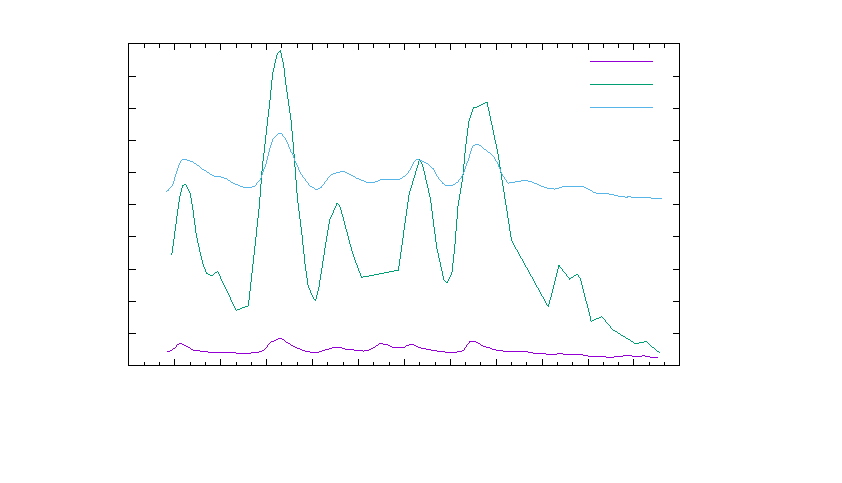
\includegraphics{../images/mercedes}}%
    \gplfronttext
  \end{picture}%
\endgroup

  \caption{Timeseries of the uncorrected \ch{NO2}, \ch{NO_x} and
    \ch{CO2} concentrations in the plume of a Mercedes B180 CDI.}
  \label{fig:mercedes-ts}
\end{figure}

\begin{figure}[htbp]
  \centering
  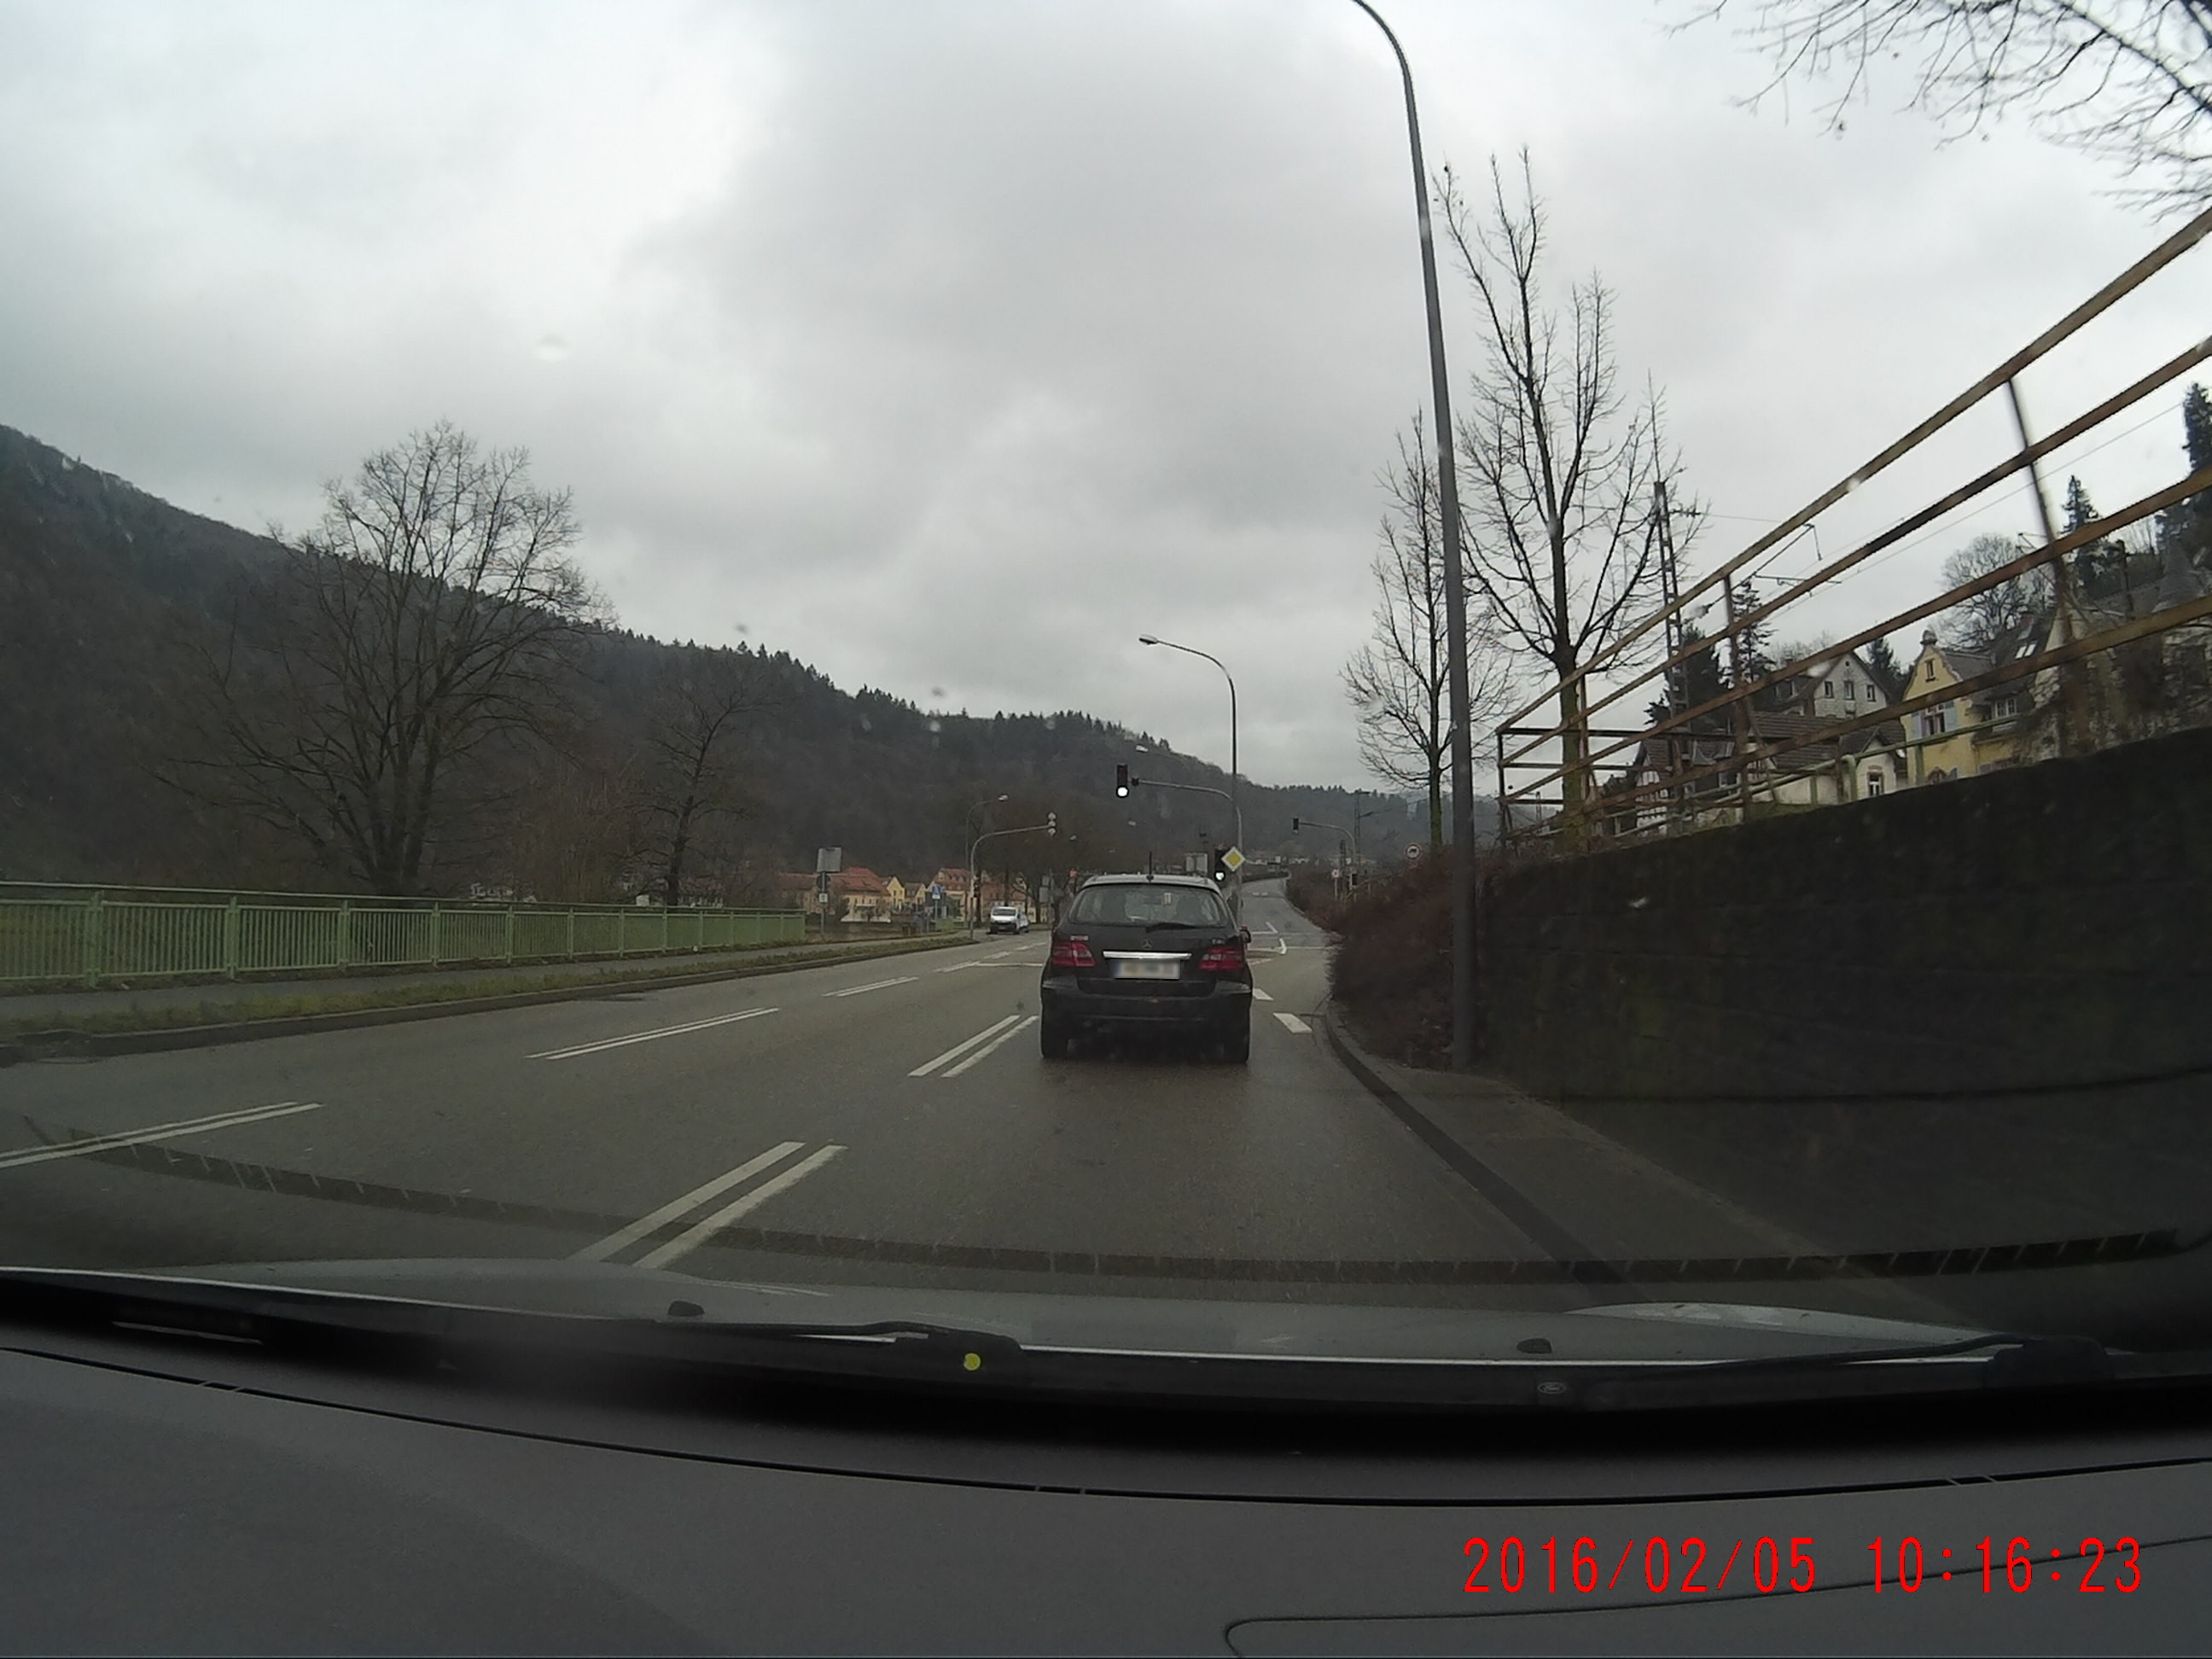
\includegraphics[width=0.45\textwidth]{mercedes.jpg}
  \hfill  
  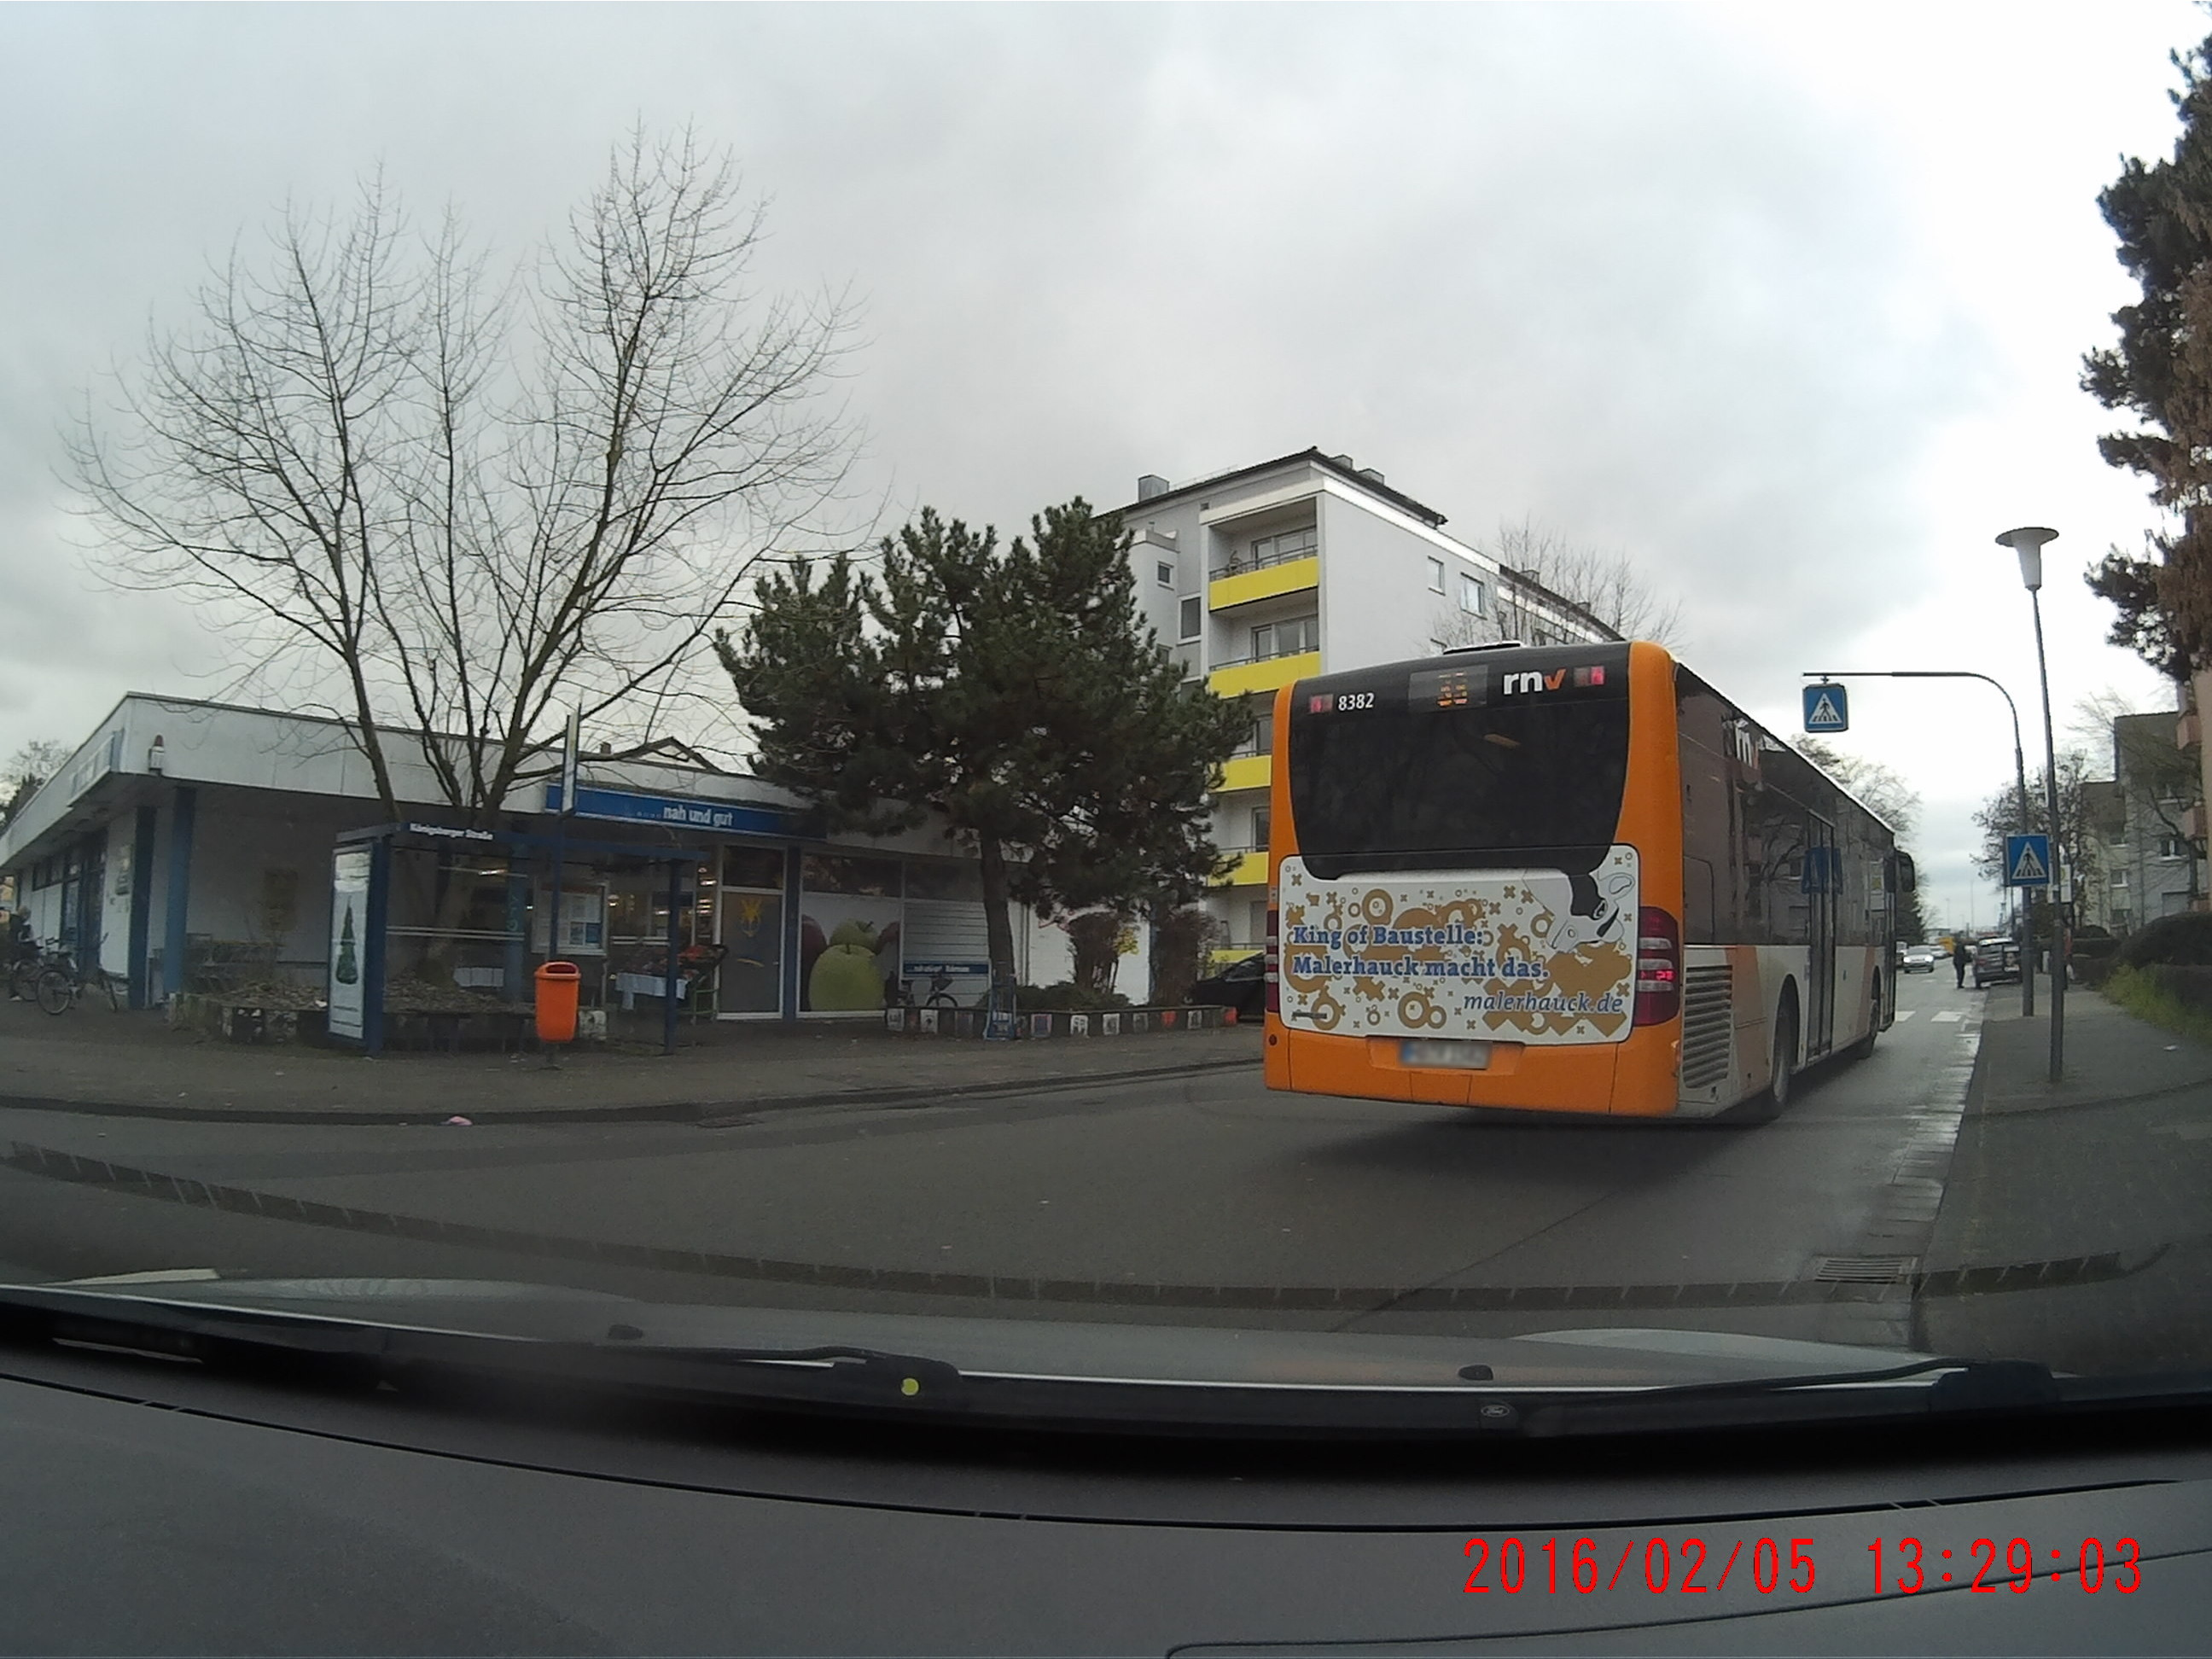
\includegraphics[width=0.45\textwidth]{bus.jpg}
  \caption{Picture of the measured bus and Mercedes B180 CDI.\@{}Please note that
    the printed time is in utc.}
  \label{fig:bus}
\end{figure}

\begin{table}[hbtp]
  \centering
  \begin{tabular}{l S S}
    \toprule
    & {Mercedes} & {Bus}\\
    \midrule
    \ch{NO2}/\ch{CO2} & 2.2(3)e-4 & 6(2)e-4\\
    \ch{NO_x}/\ch{CO2}& 5.0(7)e-3 & 6(1)e-3\\
    \bottomrule
  \end{tabular}
  \caption{\ch{NO2} and \ch{NO_x} to \ch{CO2} ratios for the two
    vehicles.}
  \label{tab:mercedes-bus}
\end{table}

\begin{figure}[htbp]
  \centering
  % GNUPLOT: LaTeX picture with Postscript
\begingroup
  \makeatletter
  \providecommand\color[2][]{%
    \GenericError{(gnuplot) \space\space\space\@spaces}{%
      Package color not loaded in conjunction with
      terminal option `colourtext'%
    }{See the gnuplot documentation for explanation.%
    }{Either use 'blacktext' in gnuplot or load the package
      color.sty in LaTeX.}%
    \renewcommand\color[2][]{}%
  }%
  \providecommand\includegraphics[2][]{%
    \GenericError{(gnuplot) \space\space\space\@spaces}{%
      Package graphicx or graphics not loaded%
    }{See the gnuplot documentation for explanation.%
    }{The gnuplot epslatex terminal needs graphicx.sty or graphics.sty.}%
    \renewcommand\includegraphics[2][]{}%
  }%
  \providecommand\rotatebox[2]{#2}%
  \@ifundefined{ifGPcolor}{%
    \newif\ifGPcolor
    \GPcolorfalse
  }{}%
  \@ifundefined{ifGPblacktext}{%
    \newif\ifGPblacktext
    \GPblacktexttrue
  }{}%
  % define a \g@addto@macro without @ in the name:
  \let\gplgaddtomacro\g@addto@macro
  % define empty templates for all commands taking text:
  \gdef\gplbacktext{}%
  \gdef\gplfronttext{}%
  \makeatother
  \ifGPblacktext
    % no textcolor at all
    \def\colorrgb#1{}%
    \def\colorgray#1{}%
  \else
    % gray or color?
    \ifGPcolor
      \def\colorrgb#1{\color[rgb]{#1}}%
      \def\colorgray#1{\color[gray]{#1}}%
      \expandafter\def\csname LTw\endcsname{\color{white}}%
      \expandafter\def\csname LTb\endcsname{\color{black}}%
      \expandafter\def\csname LTa\endcsname{\color{black}}%
      \expandafter\def\csname LT0\endcsname{\color[rgb]{1,0,0}}%
      \expandafter\def\csname LT1\endcsname{\color[rgb]{0,1,0}}%
      \expandafter\def\csname LT2\endcsname{\color[rgb]{0,0,1}}%
      \expandafter\def\csname LT3\endcsname{\color[rgb]{1,0,1}}%
      \expandafter\def\csname LT4\endcsname{\color[rgb]{0,1,1}}%
      \expandafter\def\csname LT5\endcsname{\color[rgb]{1,1,0}}%
      \expandafter\def\csname LT6\endcsname{\color[rgb]{0,0,0}}%
      \expandafter\def\csname LT7\endcsname{\color[rgb]{1,0.3,0}}%
      \expandafter\def\csname LT8\endcsname{\color[rgb]{0.5,0.5,0.5}}%
    \else
      % gray
      \def\colorrgb#1{\color{black}}%
      \def\colorgray#1{\color[gray]{#1}}%
      \expandafter\def\csname LTw\endcsname{\color{white}}%
      \expandafter\def\csname LTb\endcsname{\color{black}}%
      \expandafter\def\csname LTa\endcsname{\color{black}}%
      \expandafter\def\csname LT0\endcsname{\color{black}}%
      \expandafter\def\csname LT1\endcsname{\color{black}}%
      \expandafter\def\csname LT2\endcsname{\color{black}}%
      \expandafter\def\csname LT3\endcsname{\color{black}}%
      \expandafter\def\csname LT4\endcsname{\color{black}}%
      \expandafter\def\csname LT5\endcsname{\color{black}}%
      \expandafter\def\csname LT6\endcsname{\color{black}}%
      \expandafter\def\csname LT7\endcsname{\color{black}}%
      \expandafter\def\csname LT8\endcsname{\color{black}}%
    \fi
  \fi
    \setlength{\unitlength}{0.0500bp}%
    \ifx\gptboxheight\undefined%
      \newlength{\gptboxheight}%
      \newlength{\gptboxwidth}%
      \newsavebox{\gptboxtext}%
    \fi%
    \setlength{\fboxrule}{0.5pt}%
    \setlength{\fboxsep}{1pt}%
\begin{picture}(7200.00,5040.00)%
    \gplgaddtomacro\gplbacktext{%
      \csname LTb\endcsname%
      \put(946,966){\makebox(0,0)[r]{\strut{}$0$}}%
      \put(946,1389){\makebox(0,0)[r]{\strut{}$500$}}%
      \put(946,1812){\makebox(0,0)[r]{\strut{}$1000$}}%
      \put(946,2236){\makebox(0,0)[r]{\strut{}$1500$}}%
      \put(946,2659){\makebox(0,0)[r]{\strut{}$2000$}}%
      \put(946,3082){\makebox(0,0)[r]{\strut{}$2500$}}%
      \put(946,3505){\makebox(0,0)[r]{\strut{}$3000$}}%
      \put(946,3929){\makebox(0,0)[r]{\strut{}$3500$}}%
      \put(946,4352){\makebox(0,0)[r]{\strut{}$4000$}}%
      \put(946,4775){\makebox(0,0)[r]{\strut{}$4500$}}%
      \put(1078,834){\rotatebox{-45}{\makebox(0,0)[l]{\strut{}14:25:00}}}%
      \put(1549,834){\rotatebox{-45}{\makebox(0,0)[l]{\strut{}14:26:00}}}%
      \put(2021,834){\rotatebox{-45}{\makebox(0,0)[l]{\strut{}14:27:00}}}%
      \put(2492,834){\rotatebox{-45}{\makebox(0,0)[l]{\strut{}14:28:00}}}%
      \put(2963,834){\rotatebox{-45}{\makebox(0,0)[l]{\strut{}14:29:00}}}%
      \put(3435,834){\rotatebox{-45}{\makebox(0,0)[l]{\strut{}14:30:00}}}%
      \put(3906,834){\rotatebox{-45}{\makebox(0,0)[l]{\strut{}14:31:00}}}%
      \put(4377,834){\rotatebox{-45}{\makebox(0,0)[l]{\strut{}14:32:00}}}%
      \put(4848,834){\rotatebox{-45}{\makebox(0,0)[l]{\strut{}14:33:00}}}%
      \put(5320,834){\rotatebox{-45}{\makebox(0,0)[l]{\strut{}14:34:00}}}%
      \put(5791,834){\rotatebox{-45}{\makebox(0,0)[l]{\strut{}14:35:00}}}%
      \put(5923,966){\makebox(0,0)[l]{\strut{}$0$}}%
      \put(5923,1389){\makebox(0,0)[l]{\strut{}$500$}}%
      \put(5923,1812){\makebox(0,0)[l]{\strut{}$1000$}}%
      \put(5923,2236){\makebox(0,0)[l]{\strut{}$1500$}}%
      \put(5923,2659){\makebox(0,0)[l]{\strut{}$2000$}}%
      \put(5923,3082){\makebox(0,0)[l]{\strut{}$2500$}}%
      \put(5923,3505){\makebox(0,0)[l]{\strut{}$3000$}}%
      \put(5923,3929){\makebox(0,0)[l]{\strut{}$3500$}}%
      \put(5923,4352){\makebox(0,0)[l]{\strut{}$4000$}}%
      \put(5923,4775){\makebox(0,0)[l]{\strut{}$4500$}}%
    }%
    \gplgaddtomacro\gplfronttext{%
      \csname LTb\endcsname%
      \put(176,2870){\rotatebox{-270}{\makebox(0,0){\strut{}\ch{NO2}/\ch{NO_x} Concentration [ppb]}}}%
      \put(6692,2870){\rotatebox{-270}{\makebox(0,0){\strut{}\ch{CO2} Concentration [ppm]}}}%
      \csname LTb\endcsname%
      \put(1738,4602){\makebox(0,0)[r]{\strut{}\ch{NO2}}}%
      \csname LTb\endcsname%
      \put(1738,4382){\makebox(0,0)[r]{\strut{}\ch{NO_x}}}%
      \csname LTb\endcsname%
      \put(1738,4162){\makebox(0,0)[r]{\strut{}\ch{CO2}}}%
    }%
    \gplbacktext
    \put(0,0){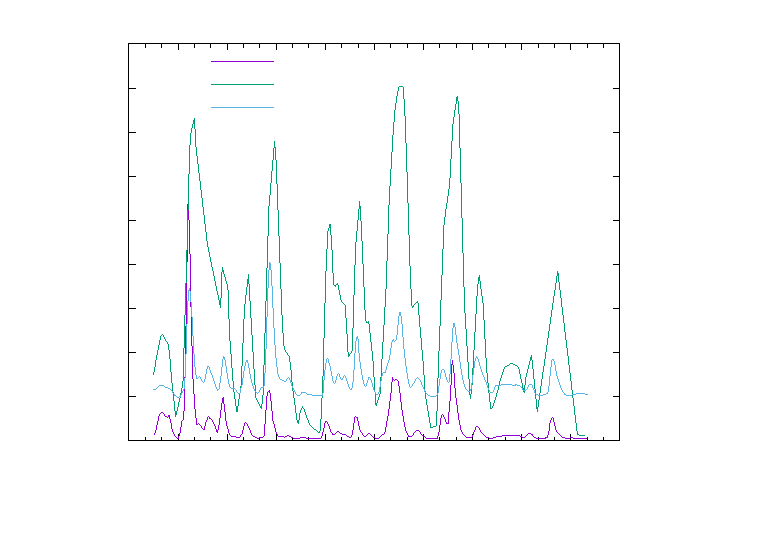
\includegraphics{../images/bus}}%
    \gplfronttext
  \end{picture}%
\endgroup

  \caption{Time series of the uncorrected \ch{NO2}, \ch{NO_x} and \ch{CO2}
    concentrations in the plume of a bus in Heidelberg.}
  \label{fig:bus-ts}
\end{figure}

The second example was the bus of the Heidelberg public-transport
system (c.\,f.\ Fig.~\ref{fig:bus} right hand side). I traced it for
\SI{10}{\minute} through mostly suburban areas with almost no
traffic. Therefore, the values depicted in the time series in
Figure~\ref{fig:bus-ts} should give a rather pure picture of the bus's
emission. During our pursuit the bus stopped at 6 bus stops, which
explain the many acceleration periods depicted. The additional ones
are due to crossroads and traffic lights. As before in the Mercedes
case, the \ch{NO_x} concentration varies the most and the \ch{CO2}
curve follows it in the same general form. The \ch{NO2} concentration
is the most stable, but shows still a peak of over \SI{2500}{ppb}. In
absolute terms, the bus has a factor 2 to 3 higher
\ch{NO_x} emission peaks than the Mercedes. During the short periods
of time in between bus stops, the emission drops drastically and is in
a comparable range to the valleys of the Mercedes time series,
however, since there are so many bus stops on the route the emission
during acceleration makes up the major part of the pollution. Looking
at the ratios in Table~\ref{tab:mercedes-bus} yield that the bus has
a three times higher \ch{NO2} ratio, but the \ch{NO_x} ratios do not
differ within the uncertainties. This can be explained by realizing
that the bus naturally has a far higher consumption than an average
street car. This directly leads to higher emissions, especialle higher
\ch{CO2} emissions, which cancel out the larger nitrogen (di-)oxide
values.

All in all these measurements yield two important take home
messages. First of all, there is further evidence that our converter
works and that it produces additional detectable \ch{NO2} in the
cavity. An interesting question for further investigation would be to
find out, whether the converter is fast enough to completely convert
\ch{NO_x} peaks with a maximum of over \SI{3500}{ppb}. Dealing with
such magnitudes (as is realistic as shown in the Bus case), the
converter could run in a region where the ozone concentration cannot
be assumed to be constant anymore and the reaction speed should
diminish. Since the conversion ratio cannot be computed exactly in
this bounding case, but should be lower than the approximated value
computed in Sectin~\ref{sec:requirements}, the above \ch{NO_x} values
should be handled with care and be understood as a lower bound for the
emission. In any case, the second important message is, that portable
\ch{NO} measurement instruments are important for in vivo vehicle
measurements, as pure \ch{NO2} instruments may underestimate the
\ch{NO_x} emission by a factor of 10.

%%% Local Variables:
%%% mode: latex
%%% TeX-master: "../Bachelor"
%%% End:
